% This is a Basic Assignment Paper but with like Code and stuff allowed in it, there is also url, hyperlinks from contents included. 

\documentclass[11pt]{article}

% Preamble

\usepackage[margin=1in]{geometry}
\usepackage{amsfonts, amsmath, amssymb}
\usepackage{fancyhdr, float, graphicx}
\usepackage[utf8]{inputenc} % Required for inputting international characters
\usepackage[T1]{fontenc} % Output font encoding for international characters
\usepackage{fouriernc} % Use the New Century Schoolbook font
\usepackage[nottoc, notlot, notlof]{tocbibind}
\usepackage{listings}
\usepackage{xcolor}
\usepackage{blindtext}
\usepackage{hyperref}
\hypersetup{
    colorlinks=true,
    linkcolor=black,
    filecolor=magenta,      
    urlcolor=cyan,
    pdfpagemode=FullScreen,
    }

\definecolor{codegreen}{rgb}{0,0.6,0}
\definecolor{codegray}{rgb}{0.5,0.5,0.5}
\definecolor{codepurple}{rgb}{0.58,0,0.82}
\definecolor{backcolour}{rgb}{0.95,0.95,0.92}

\lstdefinestyle{mystyle}{
    backgroundcolor=\color{backcolour},   
    commentstyle=\color{codegreen},
    keywordstyle=\color{magenta},
    numberstyle=\tiny\color{codegray},
    stringstyle=\color{codepurple},
    basicstyle=\ttfamily\footnotesize,
    breakatwhitespace=false,         
    breaklines=true,                 
    captionpos=b,                    
    keepspaces=true,                 
    numbers=left,                    
    numbersep=5pt,                  
    showspaces=false,                
    showstringspaces=false,
    showtabs=false,                  
    tabsize=2
}

\lstset{style=mystyle}

% Header and Footer
\pagestyle{fancy}
\fancyhead{}
\fancyfoot{}
\fancyhead[L]{\textit{\Large{Database Management Systems Assignment 1}}}
%\fancyhead[R]{\textit{something}}
\fancyfoot[C]{\thepage}
\renewcommand{\footrulewidth}{1pt}



% Other Doc Editing
% \parindent 0ex
%\renewcommand{\baselinestretch}{1.5}

\begin{document}

\begin{titlepage}
	\centering

	%---------------------------NAMES-------------------------------

	\huge\textsc{
		MIT World Peace University
	}\\

	\vspace{0.75\baselineskip} % space after Uni Name

	\LARGE{
		Database Management Systems\\
		Second Year B. Tech, Semester 4
	}

	\vfill % space after Sub Name

	%--------------------------TITLE-------------------------------

	\rule{\textwidth}{1.6pt}\vspace*{-\baselineskip}\vspace*{2pt}
	\rule{\textwidth}{0.6pt}
	\vspace{0.75\baselineskip} % Whitespace above the title



	\huge{\textsc{
			Designing of Entity Relationship Diagram
		}} \\



	\vspace{0.5\baselineskip} % Whitespace below the title
	\rule{\textwidth}{0.6pt}\vspace*{-\baselineskip}\vspace*{2.8pt}
	\rule{\textwidth}{1.6pt}

	\vspace{1\baselineskip} % Whitespace after the title block

	%--------------------------SUBTITLE --------------------------	

	\LARGE\textsc{
		Assignment No. 1
	} % Subtitle or further description
	\vfill

	%--------------------------AUTHOR-------------------------------

	Prepared By
	\vspace{0.5\baselineskip} % Whitespace before the editors

	\Large{
		Krishnaraj Thadesar \\
		Cyber Security and Forensics\\
		Batch A1, PA 20
	}


	\vspace{0.5\baselineskip} % Whitespace below the editor list
	\today

\end{titlepage}

\tableofcontents
\thispagestyle{empty}
\clearpage

\setcounter{page}{1}

\section{Aim}
Design an ER diagram for different case studies.

\section{Objectives}
To study creation of an ER diagram.

\section{Problem Statement}
Requirements of the Company
The Company is organized into:
\begin{enumerate}
	\item DEPARTMENTs. Each department has a name, number and an employee who manages the department. We keep track of the start date of the department manager.
	\item Each department controls a number of PROJECTS. Each project has a name, Number, and is located at a single location.
	\item We store each EMPLOYEEs social security number, address, salary, sex and birthdate. Each employee works for one department but may work on several projects. We keep track of the number of hours per week that an employee currently works on each project. We also keep track of the direct supervisor of each employee.
	\item Each employee may have a number of DEPENDENTS. For each dependent we keep track of their name, sex, birthdate, and relationship to the employee.
\end{enumerate}

\section{Theory}

\subsection{Entity Relationship Diagram Definition}
\begin{quote}
	\textit{	An ER diagram is a graphical representation of entities and their relationships to each other, typically used in computing in regard to the organization of data within databases or information systems. It is often used to depict the logical structure of databases and information systems.}
\end{quote}

\subsection{Entities}
\begin{quote}
	\textit{An entity is a person, place or thing. It is a thing that can be distinguished from other things. It is an object or concept about which data is stored. An entity is a noun (for example, customer, employee, product, or order). The entity is the basic building block of the data model. The entity is the object that is represented in the database. An entity is a thing that exists independently of any other thing. Entities are the nouns in the problem domain.}
\end{quote}

\subsection{Relationships}
\begin{quote}
	\textit{A relationship is a link between two or more entities. The relationship is the verb in the problem domain. The relationship is the association between two entities. Relationships are the verbs in the problem domain.}
\end{quote}

\subsubsection{Binary Relationship}
\begin{quote}
	\textit{A binary relationship is a relationship between two entities. }
\end{quote}
\subsubsection{Unary Relationship}
\begin{quote}
	\textit{A unary relationship is a relationship between one entity. }
\end{quote}
\subsubsection{Ternary Relationship}
\begin{quote}
	\textit{A ternary relationship is a relationship between three entities.}
\end{quote}

\subsection{Attributes}
\begin{quote}
	\textit{An attribute is a characteristic or quality of an entity or relationship. Attributes are the adjectives in the problem domain. Attributes are the properties of an entity or relationship. An attribute is a property of an entity that can be assigned a value. Attributes are the adjectives in the problem domain.}
\end{quote}

\subsection{Cardinality}
\begin{quote}
	\textit{Cardinality is the number of occurrences of an entity or relationship in a relationship set. The cardinality of a relationship is the number of occurrences of an entity in a relationship. The cardinality of a relationship is the number of occurrences of an entity in a relationship.}
\end{quote}

\subsection{Weak Entity}
\begin{quote}
	\textit{A weak entity is an entity that cannot exist on its own. It must have a relationship with another entity. A weak entity is identified by a relationship with another entity. It must use a foreign key in conjunction with its attributes to create a primary key.}
\end{quote}

\subsection{Primary Key}
\begin{quote}
	\textit{A primary key is a unique identifier for an entity.}
\end{quote}

\subsection{Foreign Key}
\begin{quote}
	\textit{A foreign key is a primary key of another entity.}
\end{quote}

\begin{figure}[H]
	\centering
	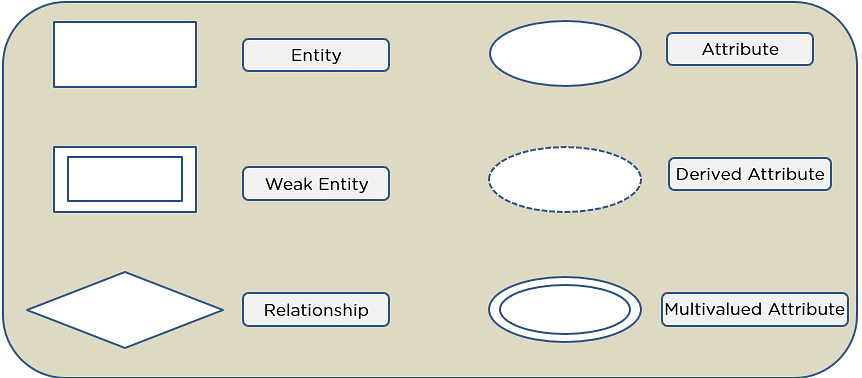
\includegraphics[scale=0.5]{ERDiagramsInDBMS_2.png}
	\caption{Symbols used in drawing ER diagrams}
\end{figure}


\section{Procedure for Drawing ER Diagram}
\begin{enumerate}
	\item Ideentify the entities
	\item Draw relationship table
	\item Draw rough er diagram.
	\item Draw each entity in depth, that have all the attributes.
	\item Show the relationship with cardinality. If it is unary ternary etc.
\end{enumerate}


\subsection{Entities in the Problem Statement}
\begin{enumerate}
	\item Company - Department
	\item Department - Name, Number, Manager, Start Date
	\item Projects - Name, Number, Location
	\item Employees - SSN, Address, Salary, sex, Birthdate, Department, Supervisor, no. of hours per week.
	\item Dependents - Name, sex, birthdate, Relationship.
\end{enumerate}

\subsection{Relationships in the Problem Statement}
\begin{figure}[H]
	\centering
	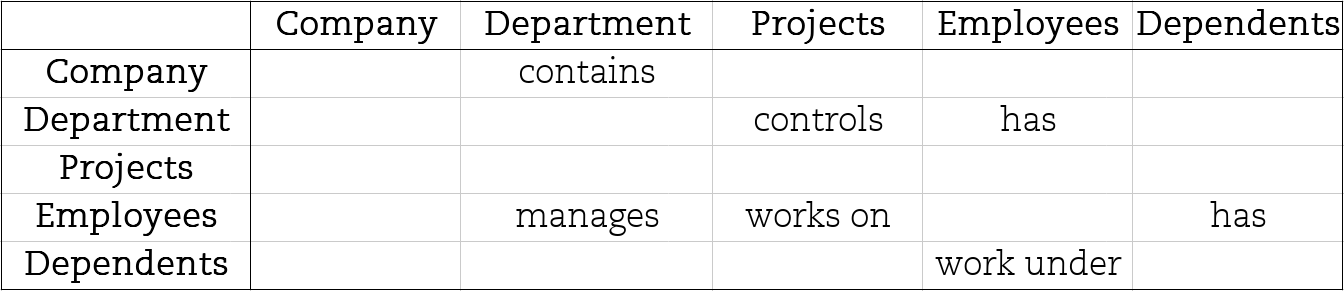
\includegraphics[scale=0.5]{table.png}
	\caption{Relationship between Entities from the Problem Statement}
\end{figure}


\section{Platform}
\textbf{Operating System}: Arch Linux x86-64 \\
\textbf{IDEs or Text Editors Used}: Draw.io for Drawing the ER diagram. \\

\section{Output}

\begin{figure}[H]
	\centering
	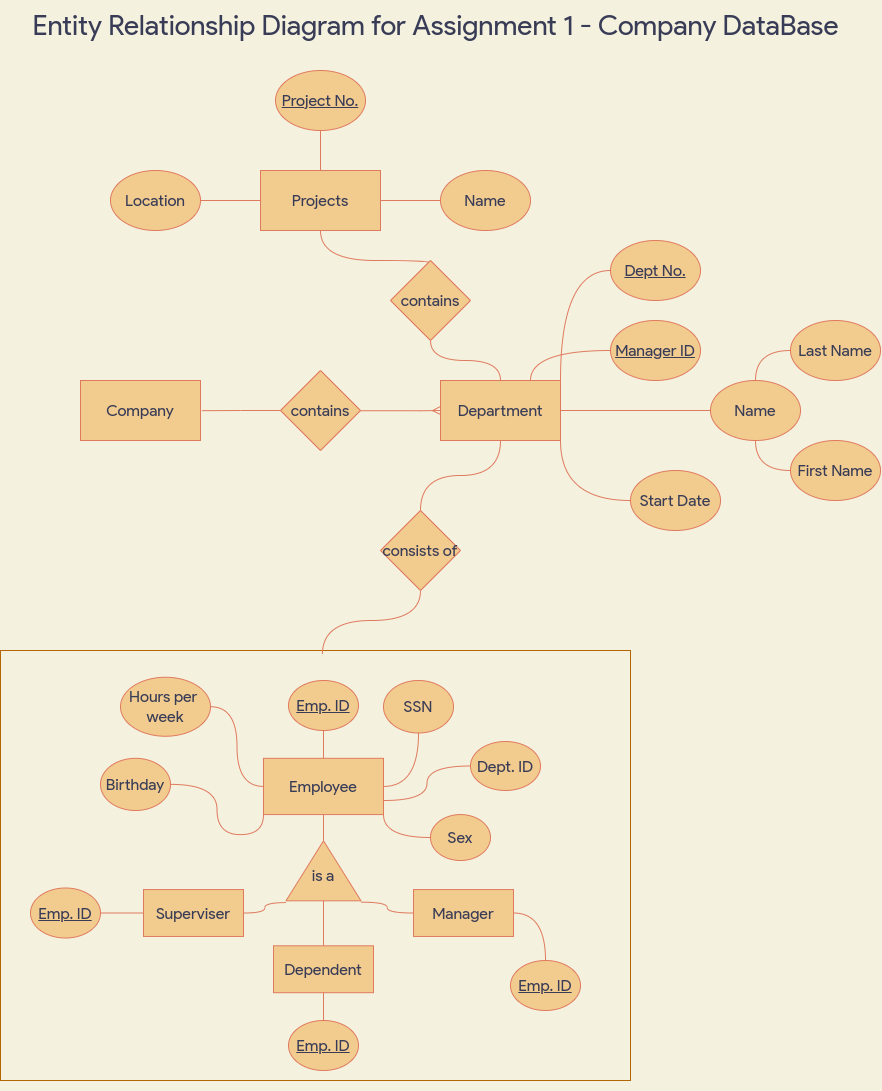
\includegraphics[scale=0.5]{./Assignment 1 ER Diagram.drawio.png}
	\caption{}
\end{figure}

\section{Conclusion}
Thus, we have learned to create ER diagram.

\section{FAQ}

\begin{enumerate}
	\item \textbf{What are different types of attributes?}

	      \begin{enumerate}
		      \item \textbf{Simple Attributes:} The attributes which are atomic in nature are called simple attributes. For example, Name, Address, Salary, etc.
		      \item \textbf{Composite Attributes:} The attributes which are not atomic in nature are called composite attributes. For example, Name of a person is a composite attribute because it is not atomic in nature. It consists of First Name, Middle Name, and Last Name.
		      \item \textbf{Multivalued Attributes:} The attributes which can have more than one value are called multivalued attributes. For example, a person can have more than one phone number. So, Phone Number is a multivalued attribute.
		      \item \textbf{Derived Attributes:} The attributes which are not stored in the database but are derived from the other attributes are called derived attributes. For example, Age is a derived attribute because it is not stored in the database but is derived from the date of birth.
		      \item \textbf{Composite Multivalued Attributes:} The attributes which are composite and multivalued are called composite multivalued attributes. For example, a person can have more than one address. So, Address is a composite multivalued attribute.
	      \end{enumerate}
	\item \textbf{What do you mean by primary key and foreign key?}

	      \begin{enumerate}
		      \item \textbf{Primary Key:} The primary key is a unique identifier for each record in a table. It is a column or a set of columns that uniquely identifies each row in a table. The primary key must contain unique values, and cannot contain NULL values. A table can have only one primary key, which may consist of single or multiple fields.
		      \item \textbf{Foreign Key:} A foreign key is a field (or collection of fields) in one table that uniquely identifies a row of another table or the same table. In simple words, the foreign key is defined in a second table, but it refers to the primary key in the first table.
	      \end{enumerate}
	\item \textbf{What is weak entity?}\\
	      \textbf{Weak Entity:} A weak entity is an entity that cannot exist on its own. It must have a relationship with another entity. A weak entity is identified by a relationship with another entity. It must use a foreign key in conjunction with its attributes to create a primary key.

	      \textbf{Example: }
	      A ROOM can only exist in a BUILDING. On the other hand, a TIRE might be considered as a strong entity because it also can exist without being attached to a CAR.
\end{enumerate}


\end{document}